\section{Physarum Polycephalum}
\label{section:background_physarum}

The organism being a subject for this work is \textit{Physarum Polycephalum} also called the many-headed slime mould. It is a member of the \textit{Physaridae} family of slime moulds, in order of \textit{Physarales}, class \textit{Myxogastria}, phylum \textit{Myxomycete}, supergroup \textit{Amoebozoa} in \textit{Protista} kingdom. While current position in taxology is well defined, presented characteristics should justify why scientists used to have problems with classification of the Physarum \cite{stephenson1994myxomycetes}.

In order to make the thesis readable, terms \textit{Physarum Polycephalum}, \textit{Physarum} or \textit{the slime mould} will be used interchangeably as the subject is unambiguously defined. As none of the authors have a background in biology, concepts are presented from a computer scientist's perspective in minimal, yet exhaustive, form.


\subsection{Biological characteristics}

\textit{Physarum Polycephalum} is a very peculiar organism. Even being a \textit{Protista} it can be observed with a naked eye --- it is a one amongst biggest living unicellular ogranisms \cite{stephenson1994myxomycetes}. 

In its natural habitat, under cool, dark and humid conditions the slime mould exists in form of a yellow semistructurized blob (as seen in figure \ref{figure:bp_habitat}). Its occurrence is fairly common around the globe, however species \textit{Physarum Polycephalum} does not occur naturally in Poland \cite{narkiewicz2013grzyby}. It feeds on bacteria, fungi and other sources of basic nutrients.

In labaratory conditions, \textit{Physarum} is stored on Petri dishes filled with non-nutritious agar (figure \ref{figure:bp_petri}). The agar base provides humid environment required for supporting plasmodial stage of the slime mould. A sterille oats or even soft porridge is used as controlled source of nutrients. Complete description of storage and observation protocol, among other informations, is provided in Appendix \ref{chapter:protocol}.

\begin{figure}
  \centering
  % TODO find another image
  \begin{subfigure}{0.45\textwidth}
    \centering
    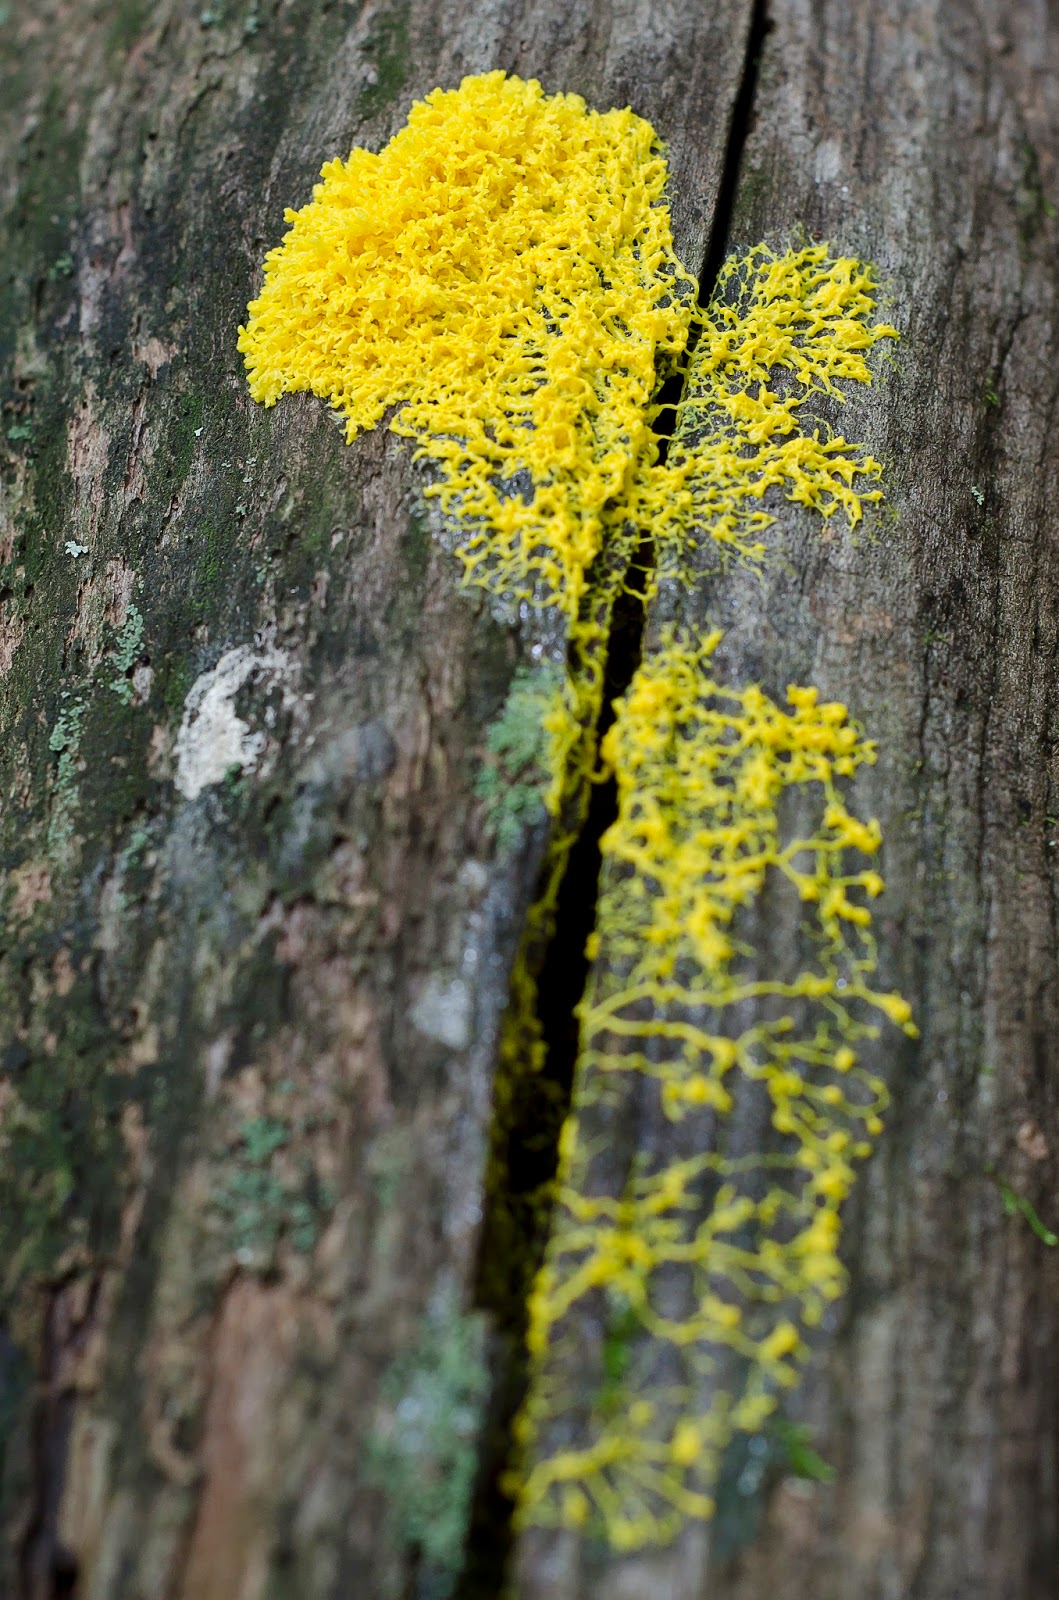
\includegraphics[width=0.44\textwidth]{background/physarum/habitat.jpg}
    \caption{Natural habitat \cite{TODO}}
    \label{figure:bp_habitat}
  \end{subfigure}
  \begin{subfigure}{0.45\textwidth}
    \centering
    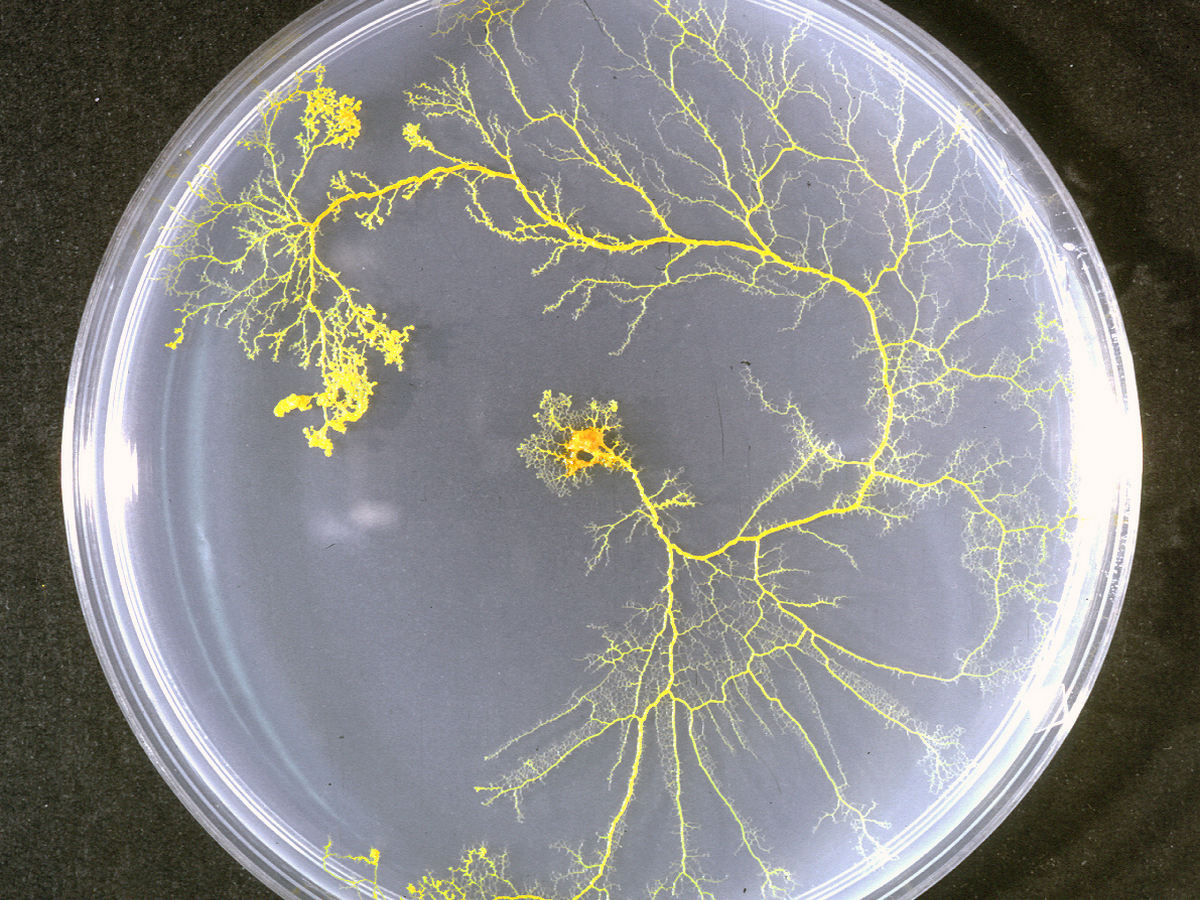
\includegraphics[width=0.9\textwidth]{background/physarum/petri.jpg}
    \caption{Petri dish}
    \label{figure:bp_petri}
  \end{subfigure}
  \caption{\textit{Physarum Polycephalum} in plasodial stage}
\end{figure}

% TODO preferred image from carolina
\begin{figure}
  \centering
  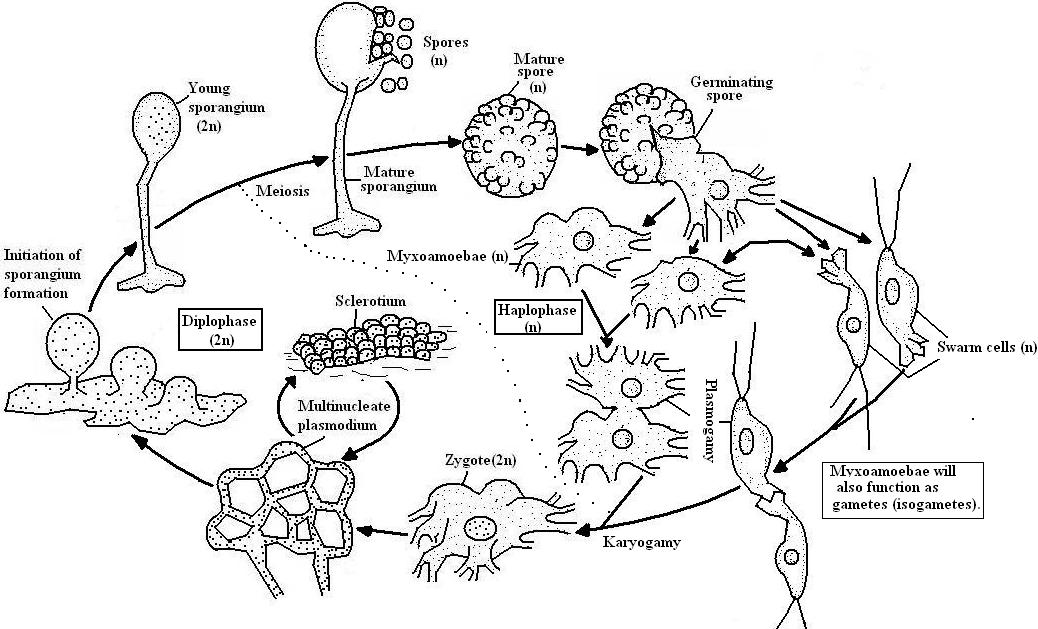
\includegraphics[width=0.94\textwidth]{background/physarum/lifecycle.png}
  \caption{Lifecycle of \textit{Physarum Polycephalum} \cite{TODO}}
  \label{figure:bp_lifecycle}
\end{figure}

As representant of \textit{Myxomycete}, a life cycle of the slime mould is very complex including haploid and diploid phases (as seen in figure \ref{figure:bp_lifecycle}). Such cycle is result of evolutionary adaptation. Formation of sporangium occurs in result of worsening conditions (such as inadequate temperature, humidity or acidity). Sporangium releases spores, which can germinate into ameboid swarm cell. Such cell can enclose itself into a cyst to protect the cells until environmental conditions improve. When conditions are favourable amoeboid cell turns into flagellated swarm cell. Swarm cells can merge, fuse their nuclei and start mitotic process resulting in forming a plasmodium \cite{jones2015pattern}.

For purposes of unconventional computing applications, \textit{Physarum} is preferred in its such plasmodial stage. However, during research transformations into other states are inevitable and must be dealt with. In case of drying and enforced starvation sclerotium is formed --- in this dormant phase \textit{Physarum Polycephalum} can survive for many years until dampness and nutrients are provided again.

Plasmodium forms protoplasmic tubes (also called pseudopodia) accordingly to food availability. Such tubes are used for discovery and transportation of nutrients. The tubes are built in similar way to animal muscles. The ectoplasm contains actin and myosin complexes, which are organised into regular structures forming tubes. Such actomyosin complexes generate contractile motion resulting in streaming of protoplasm. Furthermore, synchronized oscillations of protoplasm stream direction can observed. Nutrients are transported in one direction, after 1-2~minutes the direction is reversed. Period of this oscillation depends on environment quality and accesibility to food \cite{wohlfarth1979oscillatory} --- higher frequency oscillations are generated where nutrients available and no harmful environment exist, low frequency oscillations are caused by lack of food or as a result of unfavourable conditions. 

The plasmodium can grow around 10~mm per hour when actively exploring environment \cite{coggin1996dynamic}. While moving, plasmodium leaves polysaccharide traces (informally called slime, hence the name slime mould). Network of the protoplasmic tubes adapts, forming efficient ways of transporting nutrients, depending on their amount and quality \cite{nakagaki2004obtaining}. Usage of this behaviour is a fundamental principle for building physarum machines.


\subsection{Related works}

Since early 1960s \textit{Physarum Polycephalum} has been a subject to many biological and microbiological studies \cite{guttes1964mitotic,daniel1962method}, however it is late 70s when its computational-like behaviours have been observed \cite{wohlfarth1979oscillatory}.

% TODO artists
Research towards computational applications of the \textit{Physarum} truly started in 1990s. Nowadays, there exist two prominent research centers focusing on the slime mould --- one based in United Kingdom (Andrew Adamatzky\footnote{~\url{http://uncomp.uwe.ac.uk/adamatzky/}}, Jeff Jones\footnote{~\url{http://uncomp.uwe.ac.uk/jeff/}} from University of West England, Bristol), other one in Japan (Toshiyuki Nakagaki\footnote{~\url{http://www.cris.hokudai.ac.jp/cris/en/research/ob/ob\_innovative/nakagaki.html}}, Hokkaido University, Sapporo). Some of their works excited us about slime mould capabilities and inspired to write this thesis \cite{nakagaki2000intelligence,adamatzky2010physarum,jones2015pattern,adamatzky2007physarum}. Experiments presented here, focus on different aspects of \textit{Physarums} behaviour. Analyzing and understanding them gives impression of emerging computational power of such simple organism as a slime mould.


\subsubsection{Maze-solving capabilities}

Maze-solving or more constricted problem of finding, preferably shortest, paths is very common in practice. It has many applications and many possible algorithms are already available. Algorithms such as breadth-first search or more complex $A*$ are commonly used for solving mazes \cite{zelkowitz1979principles}, however Toshiyuki Nakagaki et al. proposed usage slime moulds' natural capabilities as unconventional solution to this problem \cite{nakagaki2000intelligence}.

In order to use \textit{Physarum} to solve a labiryth, a maze must be represented as a physical object. Such maze is modelled on a Petri dish where floor is made of non-nutrient agar and walls are made of thin plastic film (the maze used in the experiment is presented on figure \ref{figure:bp_maze_initial}). As the slime mould strictly prefers humid environment of the agar it will not pass arid walls made of plastic film. 

\begin{figure}
  \centering
  \begin{subfigure}{0.45\textwidth}
    \centering
    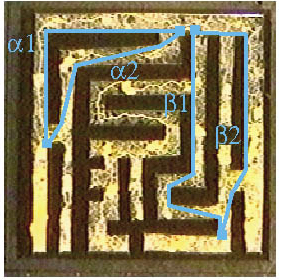
\includegraphics[width=0.9\textwidth]{background/physarum/maze1.jpg}
    \caption{Plasmodium initially filling maze}
    \label{figure:bp_maze_initial}
  \end{subfigure}
  \begin{subfigure}{0.45\textwidth}
    \centering
    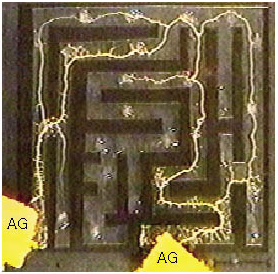
\includegraphics[width=0.9\textwidth]{background/physarum/maze2.jpg}
    \caption{Intermediate state}
    \label{figure:bp_maze_intermediate}
  \end{subfigure}
  \begin{subfigure}{0.45\textwidth}
    \centering
    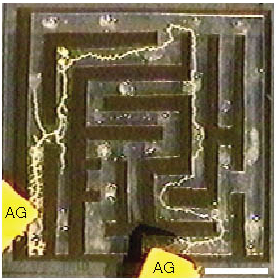
\includegraphics[width=0.9\textwidth]{background/physarum/maze3.jpg}
    \caption{Final route}
    \label{figure:bp_maze_final}
  \end{subfigure}
  \caption{\textit{Physarum} in various states of the maze experiment \cite{nakagaki2000intelligence}}
\end{figure}

There are four possible routes available $\{(\alpha_1,\beta_1), (\alpha_1,\beta_2), (\alpha_2,\beta_1), (\alpha_2,\beta_2)\}$ between entry point $A$ and exit point $B$. Oatmeal-agar based source of nutrients is planted in both entry and exit points, while large enough plasmodium is placed over whole floor of the maze. As time passes it can be observed that plasmodium retracts its body from labirth's dead-ends, leaving traces of slime where it previously has been placed (figure \ref{figure:bp_maze_intermediate}). 

As a result the slime mould rests only on direct paths connecting an entry with an exit point (figure \ref{figure:bp_maze_final}). Furthermore, it has been observed that \textit{Physarum Polycephalum} usually prefers shortest $(\alpha_2,\beta_1)$ path as it prefers most efficient way for transferring nutrients. While obtained results are satisfactory, it must be noted that whole process takes about 4~hours. 


\subsubsection{Spatial memory}

Memory is usually associated with neurological functions of brain, however it can be externalized in multiple ways, in example as pheromone trails of ants \cite{carroll1973ecology} or even notes-writing as humans do \cite{fisher1973effect}. Team of researchers from University of Sydney, demonstrated that \textit{Physarum Polycephalum} uses its slime as a form of spatial externalized memory \cite{reid2012slime}.

A common problem testing autonomous navigational skills in robotics is U-shaped trap problem \cite{chatterjee2001use}. Efficient solution of the issue requires some kind spatial memory or other navigational aids \cite{balch1993avoiding}, therefore it was a good candidate for a test of slime mould's memoizing capabilities. U-maze problem requires an agent (a robot or as in this example the slime mould) to navigate itself from starting position to the goal, where goal is hidden beside an u-shaped trap (figure \ref{figure:bp_trap_model}). The agent has to use some kind of environment map or use reactive guidance to bypass the trap (figure \ref{figure:bp_trap_model_success}), otherwise, most probably, it will be stuck inside the trap (figure \ref{figure:bp_trap_model_failure}).

% TODO create vector images like these
\begin{figure}
  \centering
  \begin{subfigure}{0.45\textwidth}
    \centering
    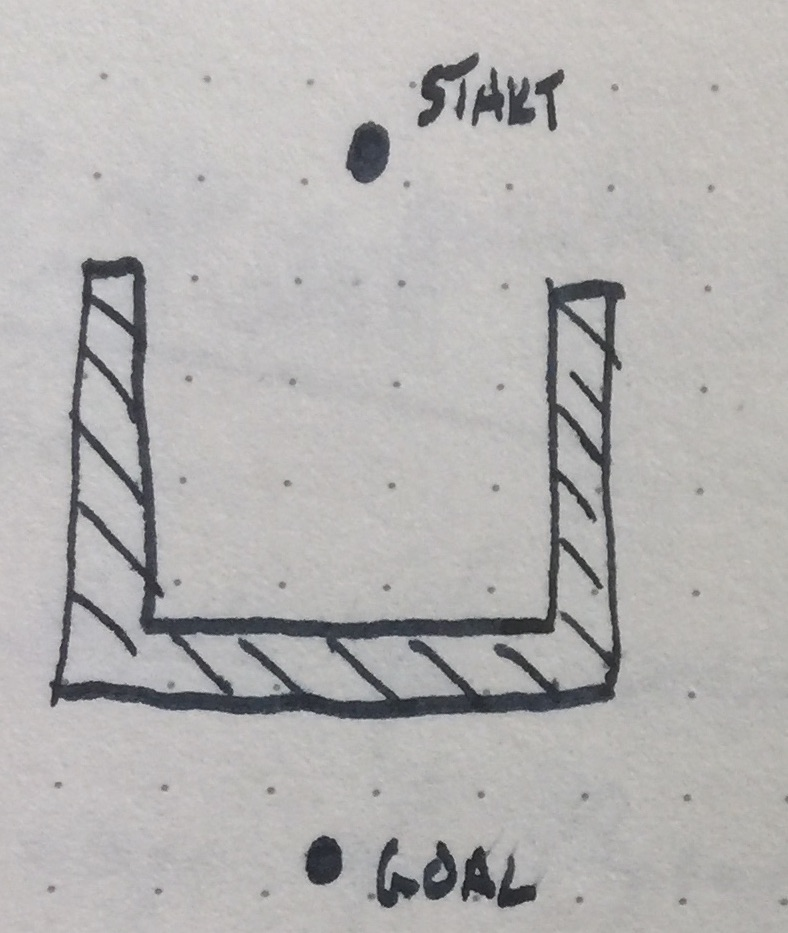
\includegraphics[width=0.9\textwidth]{background/physarum/trap_model_initial.jpg}
    \caption{Initial setup}
    \label{figure:bp_trap_model}
  \end{subfigure}
  \begin{subfigure}{0.45\textwidth}
    \centering
    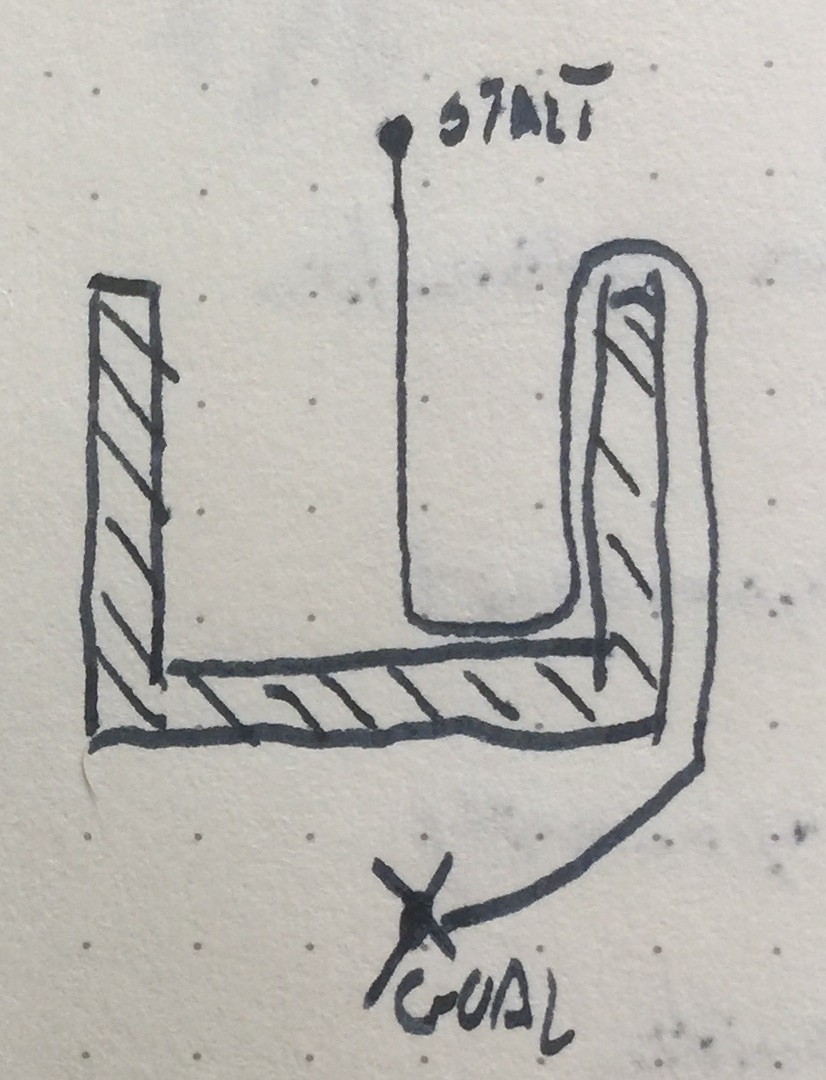
\includegraphics[width=0.9\textwidth]{background/physarum/trap_model_success.jpg}
    \caption{Example successful route to goal}
    \label{figure:bp_trap_model_success}
  \end{subfigure}
  \begin{subfigure}{0.45\textwidth}
    \centering
    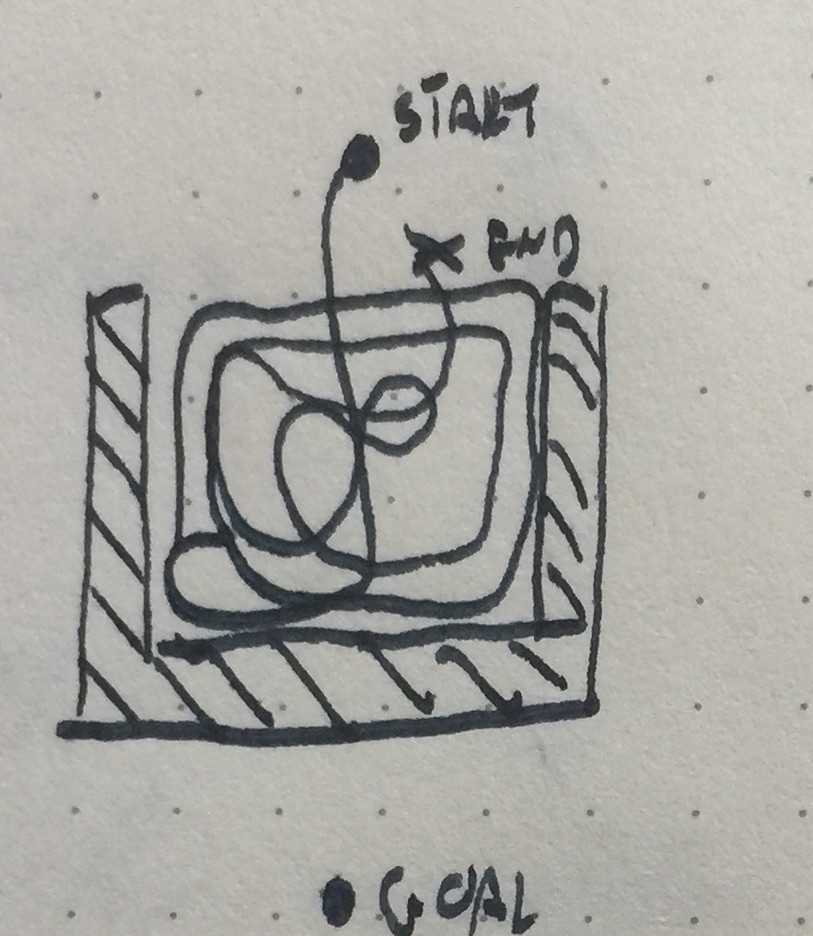
\includegraphics[width=0.9\textwidth]{background/physarum/trap_model_failure.jpg}
    \caption{Typical failure}
    \label{figure:bp_trap_model_failure}
  \end{subfigure}
  \caption{U-trap test with possible outcomes}
\end{figure}

The experiment conducted by Reid, Latty, Dussutour and Beekman \cite{reid2012slime} used \textit{Physarum Polycephalum} as an agent in non-nutrient agar environment, where the trap was made out of acetate and the goal was highly nutritious glucose. Agar base allows diffusion of glucose particles, resulting in nutrients gradient towards the goal.

Initial experiments indicated that \textit{Physarum} moves in direction where its slime is not present, however if no such direction exists (that is there is the slime all around plasmodium) it moves in random direction or all over the substrate. Therefore a slime mould has a choice to explore unexplored, however it is not an ultimate one, as it always can maneuver in previously visited areas. 

\begin{figure}
  \centering
  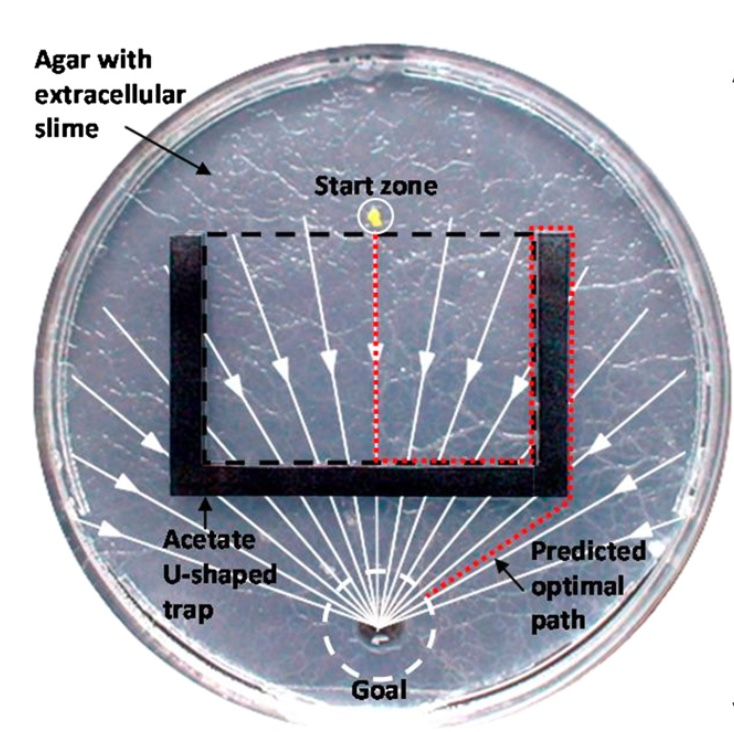
\includegraphics[width=0.74\textwidth]{background/physarum/trap_experiment.jpg}
  \caption{\textit{Physarum Polycephalum} in U-trap experiment on a slime covered substrate \cite{reid2012slime}}
  \label{figure:bp_trap_experiment}
\end{figure}

As the slime is stable, nonliving substance mostly made of galactose polymers it can be easily handled, collected and replanted \cite{mccormick1970isolation}. Two varieties of the experiment has been designed --- in a first one, previously collected slime is placed all over the substrate (figure \ref{figure:bp_trap_experiment}), where in a second one the substrate is just a clean agar. The first environment constrains \textit{Physarum} not to rely on slime for navigation (as provided slime acts as noise), unlike the second one, in which \textit{Physarum} can use the slime freely for its navigation.

Experiments have shown that \textit{Physarum} placed on a substrate already coated with the slime cannot easily escape out of the U-trap --- it spends there a long time until it leaves the trap. Furthemore, only in 33\% of 24 repeated cases plasmodium reaches the goal. However, when plasmodium is put on a clean agar substrate, an ability to use its slime as navigational aid results in reaching the goal in 96\% of cases. Both travelled distance and time to reach the goal were much shorter when the organism were able to use the slime. These findings prove that \textit{Physarum Polycephalum} can sense its extracellular slime and uses its existence as form of externalized spatial memory for recognition of previously explored areas.


\subsubsection{Adaptive network design}

Networks are used in a variety fields of engineering --- from civil roads, water pipelines, railway systems to energy grids, not to mention the Internet. Design of a useful robust network usually implies a balance between efficiency, cost and fault tolerance. Increasing robustness involves creation of redundant connections between some of the nodes. This might seem not to be profitable, however it allows network to gracefully degrade and still maintain some of its throughput. Japanese team of scientists shows \textit{Physarum Polycephalum} can be used to design networks on a par with human or algorithmic designs \cite{tero2010rules}.

% TODO remove letters from pictures
\begin{figure}
  \centering
  \begin{subfigure}{0.33\textwidth}
    \centering
    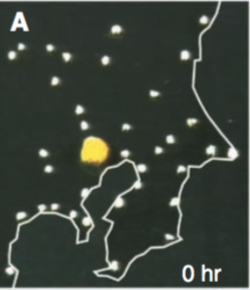
\includegraphics[width=0.9\textwidth]{background/physarum/network_initial.jpg}
    \caption{Initial placement}
    \label{figure:bp_network_initial}
  \end{subfigure}
  \begin{subfigure}{0.33\textwidth}
    \centering
    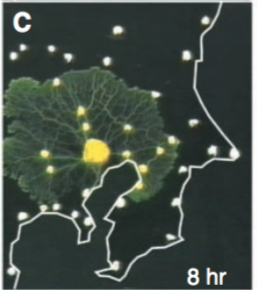
\includegraphics[width=0.9\textwidth]{background/physarum/network_intermediate_a.jpg}
    \caption{State in $t=8h$}
    \label{figure:bp_network_intermediate_a}
  \end{subfigure}
  \\
  \begin{subfigure}{0.33\textwidth}
    \centering
    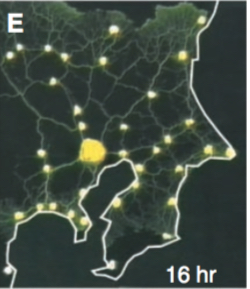
\includegraphics[width=0.9\textwidth]{background/physarum/network_intermediate_b.jpg}
    \caption{State in $t=16h$}
    \label{figure:bp_network_intermediate_b}
  \end{subfigure}
  \begin{subfigure}{0.33\textwidth}
    \centering
    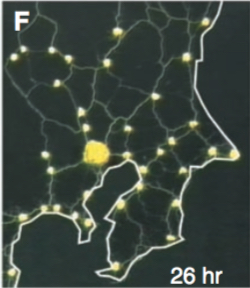
\includegraphics[width=0.9\textwidth]{background/physarum/network_final.jpg}
    \caption{Final plasmodium state}
    \label{figure:bp_network_final}
  \end{subfigure}
  \caption{Example \textit{Physarum Polycephalum} network in railway experiment \cite{tero2010rules}}
\end{figure}

The choice of the slime mould was quite natural: the organism forms a network as it forages and it can be assumed, that trough uncountable years of evolution, its designs has reached an equilibrium between cost, efficiency and robustness. The researchers prepared an experiment based on design of Tokyo-area rail network. On a substrate made of agar 36~food~sources (identical oatmeals) have been placed as in topographical positions of the rail stations (figure \ref{figure:bp_network_initial}). A blob of plasmodium has been placed where city of Tokyo would be, after some time, as the slime mould forages, it covers the substrate and connects each food source (figures \ref{figure:bp_network_intermediate_a}, \ref{figure:bp_network_intermediate_b}). Afterwards \textit{Physarum} retracts its body from the empty areas, leaving only interconnected food sources (figure \ref{figure:bp_network_final}). It should be observed, that some junctions have been left where no food is placed --- these are Steiner~points \cite{kou1981fast} enhancing overall efficiency of the network.

The experiment has been replicated 20~times, each time resulting in slightly different design of the final network, however they always resembled a Tokyo rail network designed by civil engineers. In order to even further improve similarity, the substrate has been illuminated where geographical features restrain the rail network. As the slime mould avoids light, such illumination acted as constraint for the network --- these networks bore even bigger similarities to original plans than networks made without constraints. 

In the end it was concluded that networks designed by \textit{Physarum Polycephalum} have lower overall cost with similar transport efficiency, however they lack a bit of fault tolerance --- while in only 4\% of faults the rail network would lead to isolation of any part, in case of networks designed by the slime mould such isolation would occur in 14\% of faults. Still, these results are acceptable as \textit{Physarum}'s network has much lower cost. Nonetheless, it should be noted that these networks should not be compared directly --- stops on Tokyo network have not been planned at once, they evolved as the city grew, while task given to \textit{Physarum} assumed known locations of the stops. The processes differs even more, as design of real rail network is usually centrilezed, however the slime mould acts as self-organized mechanism without central control.


\subsubsection{Slime mould models}

In the same work \cite{tero2010rules} Japanese researchers proposed a mathematical model of \textit{Physarum Polycephalum} used for adaptive network designs based on a flow network. The slime mould has been adapted as initially random lattice, where edges represents the pseudopodia. Flux inside pseudopodia has been accurrately defined with Hagen-Poiseuille formula for laminar flow \cite{sutera1993history}. Simulation is conducted in discrete time steps, in each steps a random food source node is selected to drive the flow through the network, where another food source is selected a sink. Strength of the flow influences conductibity of each tube --- unused tubes gradually disappear, while effective tubes adapts to increase throughput. This model reflects some of the properties of the real slime mould and can be used for design of adaptive network model.

Quite profound work on modelling \textit{Physarum Polycephalum} has been presented by Jeff Jones in his book \cite{jones2015pattern}. He modelled plasmodium in multi-agent fashion as a material made of multiple particles working towards reaction-diffusion process. A single agent is represents a particle of plasmodium gel/sol structure --- its movement resembles protoplasmatic flow, however when it is immobile it could be treated as gel matrix. Each agent can sense chemoattractants in two-dimensional substrate using three forward-directed sensors. A single agent can move in oscillatory or non-oscillatory modes, where first one can be used to approximate resistance within plasmodium and the second one represents ideal movement without any external forcees. Plasmodium-like behaviour emerges from collection of such randomly placed agents. Furthermore chemoattractants and chemorepellents can be placed on the substrate, stimulating the agents to regroup and move. This model can be tuned to closely resemble real \textit{Physarum Polycephalum} in a variety of environment conditions.

% TODO crop images so they are aligned
\begin{figure}
  \centering
  \begin{subfigure}{0.3\textwidth}
    \centering
    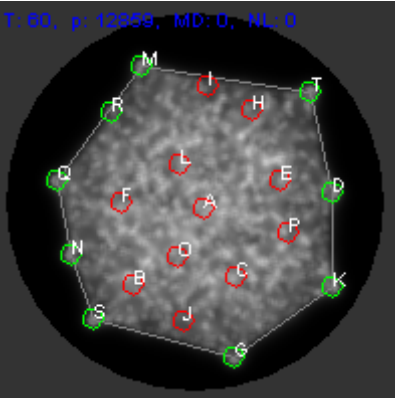
\includegraphics[width=0.9\textwidth]{background/physarum/tsp_initial.png}
    \caption{Initial placement within convex hull}
    \label{figure:bp_tsp_initial}
  \end{subfigure}
  \begin{subfigure}{0.3\textwidth}
    \centering
    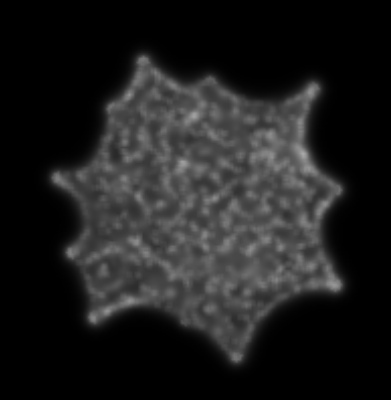
\includegraphics[width=0.9\textwidth]{background/physarum/tsp_intermediate.png}
    \caption{State after removal of some agents}
    \label{figure:bp_tsp_intermediate}
  \end{subfigure}
  \begin{subfigure}{0.3\textwidth}
    \centering
    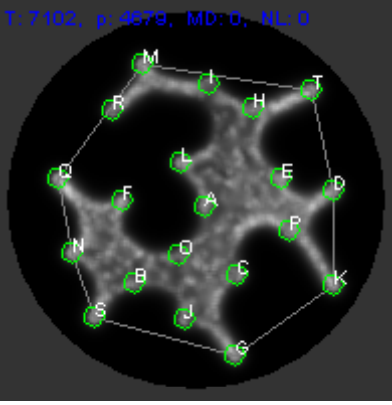
\includegraphics[width=0.9\textwidth]{background/physarum/tsp_final.png}
    \caption{Final state of simulation}
    \label{figure:bp_tsp_final}
  \end{subfigure}
  \caption{Solving TSP using shrinking blob method \cite{jones2014computation}}
\end{figure}

\begin{figure}
  \centering
  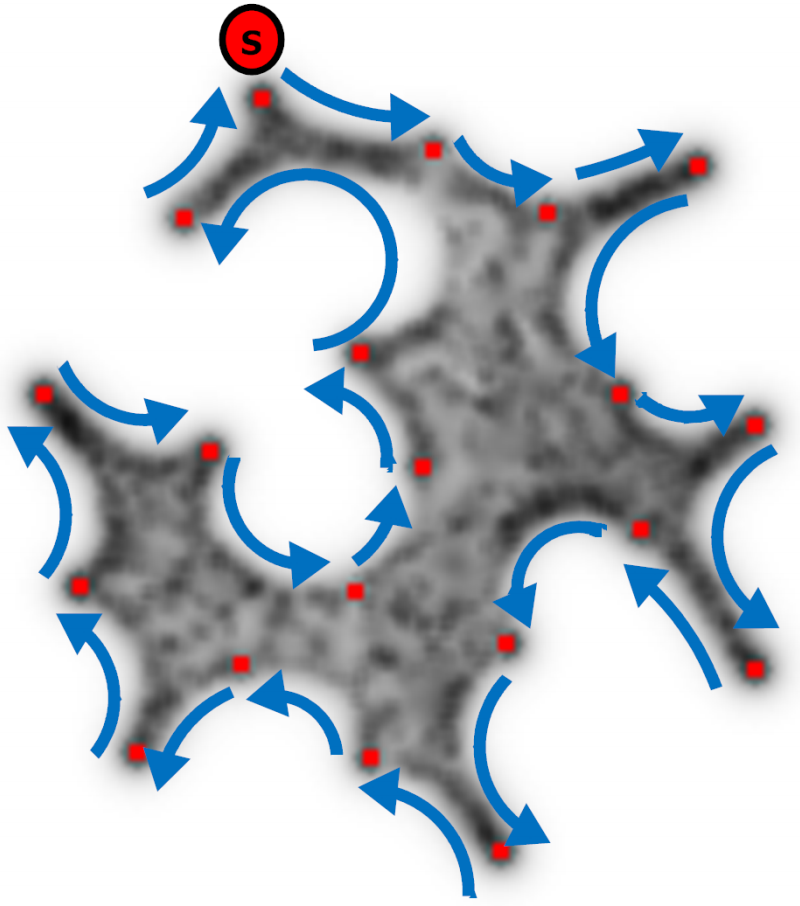
\includegraphics[width=0.3\textwidth]{background/physarum/tsp_readout.png}
  \caption{TSP tour readout method \cite{jones2014computation}}
  \label{figure:bp_tsp_readout}
\end{figure}

Based on this model Jeff Jones and Andy Adamatzky proposed a method of shrinking blob for approximating solution of Travelling Salesman Problem \cite{jones2014computation}. This method requires putting previously described agents inside a convex hull computed on topology of TSP input (figure \ref{figure:bp_tsp_initial}). Initially chemoattractants are placed nearby data points, as simulation goes some agents are removed from the virtual plasmodium, effectively shrinking the blob (figure \ref{figure:bp_tsp_intermediate}). Simulation is stopped when each node is partially uncovered --- a $5x5$ window passes over each node and checks for such condition (figure \ref{figure:bp_tsp_final}). Resulting TSP tour can be read by tracking perimeter of the blob at the end of simulation (figure \ref{figure:bp_tsp_readout}). The authors evaluated this method to be 4.27\% worse than optimal solutions in their dataset.


\subsection{Observations}

We were lucky to be in possession of \textit{Physarum Polycephalum} culture obtained from Carolina Biological Supply. The access to the living organism allowed us to observe its behaviour in variety of conditions. As for computer scientists, who have not previously done any wet lab works, it was a very educational challenge to handle alive slime mould --- detailed methods of handling are presented in Appendix \ref{chapter:protocol}.

% TODO substrates
% TODO food
% TODO movement speed
% TODO light
% TODO constraints
% TODO 3d structures
% TODO size of population, size of pseudopodia
% TODO oscillations


